\section{Fehlerbetrachtung}
\label{sec:fehler}
Für die Fehlerbetrachtung ist davon auszugehen, dass jegliche Messeinrichtungen die Messwerte mit Fehlern in bestimmten Toleranzen aufnehmen. Weiterhin sind Vereinfachungen für die auswertenden Berechnungen angenommen worden, welche die ausgewerteten Ergebnisse ebenfalls verfälschen. Die vorliegenden Ergebnisse sind demnach nur eine Näherung an den realen Zustand. Dennoch sind sie ausreichend um die qualitativen Unterschiede zwischen Reihen- und Parallelschaltung aufzuzeigen.\\
Um einen Teil der fehlerbehafteten Größen für die einzelnen Wärmetauscher zu quantifizieren bzw. die Wärmeströme entsprechend zu korrigieren, wurde für diesen Versuch ein Korrekturvolumenstrom eingeführt. Für die jeweilige Schaltung und den jeweiligen Wärmetauscher sind diese Korrekturvolumenströme im Diagramm \ref{dia:korrrek} aufgetragen. Dabei ist zu erkennen, dass der Betrag des Korrekturvolumenstroms für den \mbox{Wärmeübertrager 1} am höchsten hervorsticht. Dies sollte bei der Bewertung der berechneten Daten berücksichtigt werden.\\
Weiterhin sind Vereinfachungen getroffen worden, dass sich beispielsweise die Volumenströme in der Parallelschaltung gleichmäßig aufteilen, sowie dass für bestimmte, temperaturabhängige Größen Näherungsgleichungen genutzt wurden.

\begin{figure}[h!]
	\begin{center}
		\resizebox{0.8\textwidth}{!}{
			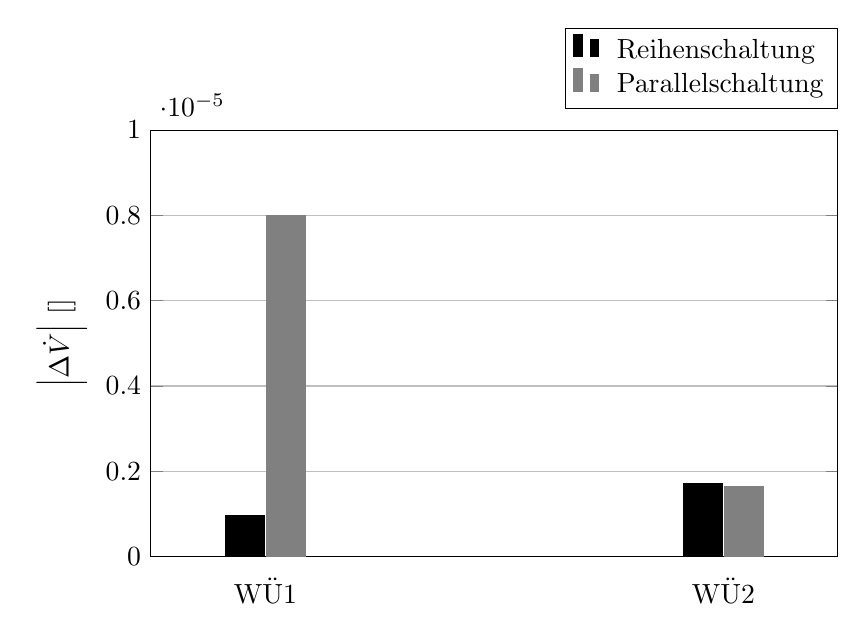
\begin{tikzpicture}
			\begin{axis}[
			width  = 0.85*\textwidth,
			height = 7cm,
			major x tick style = transparent,
			ybar=2*\pgflinewidth,
			bar width=14pt,
			ymajorgrids = true,
			ylabel = {$\left|\Delta \dot{V}\right|\, \left[\si{\cmt\per \second}\right]$},
			symbolic x coords={WÜ1,WÜ2},
			xtick = data,
			%scaled y ticks = false,
			enlarge x limits=0.25,
			ymin=0,
			ymax=0.00001,
			legend cell align=left,
			legend style={
				at={(1,1.05)},
				anchor=south east,
				column sep=1ex
			}
			]
			%Reihenschaltung
			\addplot[style={black,fill=black,mark=none}]
			coordinates {(WÜ1, 9.7E-07) (WÜ2,1.71E-06)};
			
			%Paralaleschaltung
			\addplot[style={gray,fill=gray,mark=none}]
			coordinates {(WÜ1,8.00E-06) (WÜ2,1.64E-06)};
			
			
			\legend{Reihenschaltung, Parallelschaltung}
			\end{axis}
			\end{tikzpicture}
		}
		\caption{Grafischer Vergleich der Korrekturvolumenströme}
		\label{dia:korrrek}
	\end{center}
\end{figure}
\FloatBarrier
\newpage

Auffallend für die Fehlerbetrachtung ist noch, dass die Messwerte für diesen theoretischen Versuch eine höhere Pumpleistung für die Reihen- als für Parallelleistung erfordert wird. Dies erscheint nicht als sinnvoll, da gerade durch die Aufteilung, die Lenkung und wieder Zusammenführung der Strömungen im Parallelbetrieb ein höherer Druckverlust entstehen würde als in der Reihenschaltung. Die Reihenschaltung erfordert nämlich keine Umlenkung oder Aufteilung des Fluidstroms.\\

Im Endeffekt lässt sich sagen, dass der Versuch erneut durchgeführt werden sollte, um die Ergebnisse dieses Versuches zu überprüfen. Weiterhin sollten beide Fahrweisen unter den selben Volumenströmen gefahren werden, da ein Vergleich sonst nur bedingt sinnvoll erscheint, wenn man lediglich die Schaltungen der Wärmetauscher überprüfen möchte.